% 正三棱柱示意:底面ABC,D在侧棱CC上,截面ABD;虚线DB/CB,其余实线
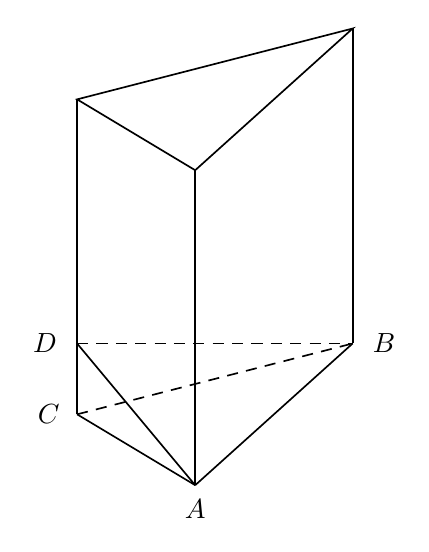
\begin{tikzpicture}[x=1cm,y=1cm,font=\normalsize,line width=.6pt,
  solid edge/.style={solid,line width=.6pt},
  hidden edge/.style={dashed,line width=.6pt,dash pattern=on 4pt off 3pt},
  geom label/.style={font=\normalsize,inner sep=2pt}]
\coordinate (A) at (0.0,0.0);
\coordinate (C) at (-1.5,0.9);
\coordinate (B) at (2.0,1.8);
\coordinate (D) at (-1.5,1.8);
\coordinate (Atop) at (0.0,4.0);
\coordinate (Ctop) at (-1.5,4.9);
\coordinate (Btop) at (2,5.8);
% bottom base
\draw[solid edge] (A) -- (C);
\draw[solid edge] (A) -- (B);
\draw[hidden edge] (C) -- (B);
% lateral edges
\draw[solid edge] (A) -- (Atop);
\draw[solid edge] (B) -- (Btop);
\draw[solid edge] (C) -- (D) -- (Ctop);
% top base
\draw[solid edge] (Ctop) -- (Atop) -- (Btop) -- cycle;
% section ABD
\draw[solid edge] (A) -- (D);
\draw[hidden edge] (D) -- (B);
% labels with clearance
\node[geom label,below] at ([yshift=-3pt]A) {$A$};
\node[geom label,left] at ([xshift=-4pt]C) {$C$};
\node[geom label,left] at ([xshift=-5pt]D) {$D$};
\node[geom label,right] at ([xshift=5pt]B) {$B$};
\end{tikzpicture}
